\scanpage{28}
\mspage{\handwritten{\unsure{2|7}2}}
% archive sheet number: 27 (inverted at the upper right)
% The long vertical cancellation crosses both paragraphs and the footnote.
% Its source extent is approximately (846,259) to the lower footnote; the pale lower continuation reaches about (725,2120).
\figure{\begin{tikzpicture}[remember picture,overlay]
\coordinate (p28cancelstart) at (5.8,-1.0);
\end{tikzpicture}}

\deleted{un morphisme de topos $\mathrm{u}:\mathrm{E}\handwritten{\longrightarrow}\mathrm{E}'$, et ce dernier sera ``unique à isomorphisme unique près'' en termes de la donnée $\mathrm{u}^{\handwritten{*}}$ resp. $\begin{tikzpicture}[baseline=(p28openingus.base),x=1em,y=1ex]
\node[inner sep=0pt] (p28openingus) at (0,0) {$\mathrm{u}_{\handwritten{*}}$};
\node[inner sep=0pt] at (.61,1.25) {\unsure{\begin{tikzpicture}[x=1em,y=1ex]\draw[gray,line width=.25pt] (0,0)--(.015,.35);\end{tikzpicture}}};
\end{tikzpicture}$, en un sens assez clair, et qui sera d'ailleurs entièrement explicité plus bas \handwritten{(\deleted{\unsure{2|3}}3.2.1)}}
% The pale short stroke above/right of the second u is kept separately; ink versus surface trace is uncertain.

\deleted{\deleted{\unsure{2|3}}\handwritten{3}.1.2. Si $\mathrm{u}:\mathrm{E}\handwritten{\longrightarrow}\mathrm{E}'$ est un morphisme de topos, il résulte des propriétés des foncteurs adjoints
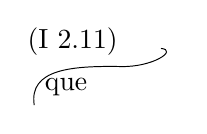
\begin{tikzpicture}[baseline=(p28que.base),x=1cm,y=1cm]
\node[anchor=base west,inner sep=0pt] (p28que) at (0,0) {que};
\node[anchor=base west,inner sep=0pt] at (-.22,.53) {\inserted{\handwritten{(I 2.11)}}};
\draw[line width=.35pt] (-.13,-.19) .. controls (-.20,.27) and (.35,.31) .. (.97,.30) .. controls (1.38,.29) and (1.70,.51) .. (1.48,.53);
\end{tikzpicture}
le foncteur image directe $\mathrm{u}_{\handwritten{*}}:\mathrm{E}\handwritten{\longrightarrow}\mathrm{E}'$ commute aux limites projectives, et le foncteur $\mathrm{u}^{\handwritten{*}}:\mathrm{E}'\handwritten{\longrightarrow}\mathrm{E}$ commute aux limites inductives
\margin{\handwritten{\deleted{\unsure{(I 2.11)|(I 4.11)|(I 4.1)}}.}}
\deleted{\unsure{(2.11)|(2.1)|(I 2.11)}}\handwritten{(${}^{*}$)}.Comme on suppose de plus que ce dernier
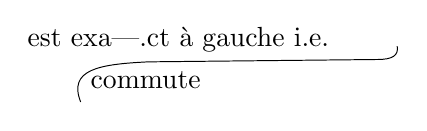
\begin{tikzpicture}[baseline=(p28commute.base),x=1cm,y=1cm]
\node[anchor=base west,inner sep=0pt] (p28commute) at (0,0) {commute};
\node[anchor=base west,inner sep=0pt] at (-.80,.53) {\inserted{\handwritten{est ex\unsure{a|.}ct à gauche i.e.}}};
\draw[line width=.35pt] (-.12,-.17) .. controls (-.28,.24) and (.10,.31) .. (.74,.34) -- (3.65,.37) .. controls (3.84,.37) and (3.92,.42) .. (3.90,.54);
\end{tikzpicture}
aux limites projectives finies, on voit donc en particulier que $\mathrm{u}^{\handwritten{*}}$ \uline{est} \deleted{exac} \uline{exact}.
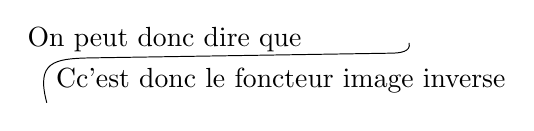
\begin{tikzpicture}[baseline=(p28cest.base),x=1cm,y=1cm]
\node[anchor=base west,inner sep=0pt] (p28cest) at (0,0) {\uline{\deleted{C}\handwritten{c}'est \deleted{donc} le foncteur image inverse}};
\node[anchor=base west,inner sep=0pt] at (-.36,.52) {\inserted{On peut donc dire que}};
\draw[line width=.35pt] (-.11,-.19) .. controls (-.25,.33) and (-.02,.37) .. (.43,.38) -- (4.25,.44) .. controls (4.38,.44) and (4.52,.46) .. (4.49,.57);
\end{tikzpicture}
$\mathrm{u}^{\handwritten{\begin{tikzpicture}[x=.1cm,y=.1cm,baseline=0pt]
\draw[line width=.35pt] (0,.9)--(.6,-.6);
\draw[line width=.35pt] (.6,1)--(-.35,-.8);
\draw[line width=.35pt] (-.15,.1)--(1.3,.1);
\fill (.55,-1.0) circle (.11);
\end{tikzpicture}}}$ \deleted{qui}, dans le couple $(\mathrm{u}_{\handwritten{*}},\mathrm{u}^{\handwritten{\begin{tikzpicture}[x=.1cm,y=.1cm,baseline=0pt]
\draw[line width=.35pt] (-.20,1.0)--(.15,.05);
\draw[line width=.35pt] (-.5,0)--(1.1,0);
\draw[line width=.35pt] (.20,-.35)--(.40,-.88);
\fill (-.48,-.65) circle (.12);
\end{tikzpicture}}})$, \uline{qui possède les propriétés d'exactitude les plus remarquables}, \deleted{assurant} Ces propriétés assurent que pour toute espèce de structure algébrique
\begin{tikzpicture}[baseline=(p28quipeut.base),x=1cm,y=1cm]
\node[anchor=base west,inner sep=0pt] (p28quipeut) at (0,0) {\deleted{qui}\,\hbox{\ttfamily x}\,\deleted{peut}};
\node[anchor=base west,inner sep=0pt] at (0,.48) {\inserted{\handwritten{$\Sigma$}}};
\node[anchor=north west,inner sep=0pt] at (.11,.44) {\unsure{\begin{tikzpicture}[x=1cm,y=1cm]\draw[gray,line width=.25pt] (0,0) .. controls (.10,-.10) and (.26,-.06) .. (.42,0);\end{tikzpicture}}};
\draw[line width=.35pt] (-.12,-.18) .. controls (-.25,.20) and (.30,.25) .. (.77,.28) .. controls (1.05,.32) and (1.18,.33) .. (1.17,.49);
\end{tikzpicture}
% The standalone x cancels the otherwise blank cell between qui and peut.
% The pale lower tail of Sigma is separate from the curved insertion leader; its function is uncertain.
dont les données peuvent se décrire en termes de données de flèches entre les ensembles de base et des ensembles déduits de ceux-ci par application répétée d'opérations de limites projectives finies et de limites inductives quelconques,
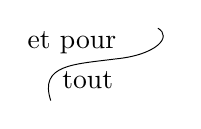
\begin{tikzpicture}[baseline=(p28tout.base),x=1cm,y=1cm]
\node[anchor=base west,inner sep=0pt] (p28tout) at (0,0) {tout};
\node[anchor=base west,inner sep=0pt] at (-.44,.50) {\inserted{\handwritten{et pour}}};
\draw[line width=.35pt] (-.14,-.16) .. controls (-.29,.30) and (.15,.30) .. (.69,.37) .. controls (1.20,.42) and (1.41,.65) .. (1.22,.76);
\end{tikzpicture}
\handwritten{``}objet de $\underline{\mathrm{E}}'$ muni d'une structure d'espèce $\handwritten{\Sigma}$'' (notion qui a un sens grâce aux propriétés d'exactitude \deleted{de} internes du topos
$\begin{tikzpicture}[baseline=(p28heavyE.base),x=1em,y=1ex]
\node[inner sep=0pt] (p28heavyE) at (0,0) {$\mathrm{E}'$};
\node[anchor=north west,inner sep=0pt] at (-.49,-.35) {\unsure{\begin{tikzpicture}[x=1em,y=1ex]\fill (0,0)--(.61,0)--(.65,-.35)--(-.02,-.35)--cycle;\end{tikzpicture}}};
\end{tikzpicture}$
% The E is definite. The thick lower impression is drawn separately: underline or displaced repeated E remains open.
(II 4.1)), son image

\begin{tikzpicture}[baseline=(p28inverse.base),x=1cm,y=1cm]
\node[anchor=base west,inner sep=0pt] (p28inverse) at (0,0) {\deleted{inverse}};
\draw[line width=.65pt] (-.08,.12)--(1.34,.12) .. controls (1.41,.12) and (1.46,.28) .. (1.50,.37);
\draw[line width=.55pt] (.02,-.12)--(.07,.38);
\end{tikzpicture}
par $\mathrm{u}^{\handwritten{*}}$ est muni des mêmes structures. Plutôt que d'entrer dans la tâche peu engageante de donner un sens précis à cet énoncé et de le justifier de façon formelle, nous conseillons au lecteur de
\begin{tikzpicture}[baseline=(p28se.base),x=1cm,y=1cm]
\node[anchor=base west,inner sep=0pt] (p28se) at (0,0) {se};
\node[anchor=base west,inner sep=0pt] at (-.46,.51) {\inserted{l'\begin{tikzpicture}[baseline=(p28expe.base),x=1em,y=1ex]
\node[inner sep=0pt] (p28expe) at (0,0) {e};
\node[inner sep=0pt] at (-.16,.61) {\unsure{\begin{tikzpicture}[x=1em,y=1ex]\draw[line width=.25pt] (0,.13)--(.21,-.15);\end{tikzpicture}}};
\end{tikzpicture}xpliciter et de}};
\draw[line width=.35pt] (-.13,-.18) .. controls (-.22,.30) and (-.01,.33) .. (.41,.34) -- (3.07,.37) .. controls (3.18,.37) and (3.25,.38) .. (3.24,.49);
\end{tikzpicture}
% The e is definite; a short upper-left diagonal remains an uncertain additional impression.
convaincre de sa validité pour des espèces de structure telles que celle de groupe, d'anneau, de module sur un anneau, de comodule \deleted{ou}\,\hbox{\ttfamily x}\,\deleted{de}\,\hbox{\ttfamily x}\,\deleted{bimodule} sur un anneau, de bigèbre sur un anneau, de torseur sous un groupe. (Dans ces exemples, les trois premières espèces de structure se définis}
% The two standalone x impressions cancel the blank cells after ou and de.
% The last word is cut at the right image edge after definis (accent as transcribed above); no unseen ending is supplied.
% The parenthesis is open on the source page.

\handwritten{\figure{
\begin{tikzpicture}[x=1cm,y=1cm]
\draw[line width=.4pt] (0,.03) .. controls (.8,-.08) and (1.0,-.05) .. (1.6,0) .. controls (4.8,.12) and (9.7,-.08) .. (13.0,.04) .. controls (13.5,.06) and (13.9,.10) .. (14.2,.03);
\end{tikzpicture}}}

\deleted{($\handwritten{\begin{tikzpicture}[x=.1cm,y=.1cm,baseline=0pt]
\draw[line width=.35pt] (-.4,.7)--(.6,-.6);
\draw[line width=.35pt] (.2,1)--(-.2,-.1);
\draw[line width=.35pt] (-.6,.1)--(1,.1);
\fill (-.28,-.65) circle (.12);
\end{tikzpicture}}$) \deleted{On peut} \deleted{d}\handwritten{D}'ailleurs
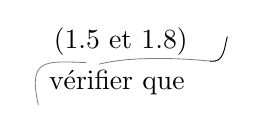
\begin{tikzpicture}[baseline=(p28verifier.base),x=1cm,y=1cm]
\node[anchor=base west,inner sep=0pt] (p28verifier) at (0,0) {\deleted{vérifier que}};
\node[anchor=base west,inner sep=0pt] at (.06,.52) {\inserted{\handwritten{(1.5 et 1.8)}}};
% Three visible leader segments: left hook, interrupted pale middle, right upturn.
\draw[gray,line width=.3pt] (-.13,-.20) .. controls (-.26,.39) and (-.06,.36) .. (.48,.34);
\draw[gray,line width=.3pt] (.64,.32) .. controls (1.04,.42) and (1.63,.40) .. (2.05,.36);
\draw[line width=.35pt] (2.05,.36) .. controls (2.23,.33) and (2.23,.52) .. (2.27,.67);
\end{tikzpicture}, pour un foncteur $\mathrm{u}_{\handwritten{\begin{tikzpicture}[x=.1cm,y=.1cm,baseline=0pt]
\draw[line width=.35pt] (-.30,.60)--(.20,.05);
\draw[line width=.35pt] (.50,.8)--(-.35,-.7);
\draw[line width=.35pt] (-.45,0)--(1,0);
\fill (.48,-.88) circle (.13);
\end{tikzpicture}}}:\mathrm{E}\handwritten{\longrightarrow}\mathrm{E}'$ resp. $\mathrm{u}^{\handwritten{\begin{tikzpicture}[x=.1cm,y=.1cm,baseline=0pt]
\draw[line width=.35pt] (-.30,.7)--(.25,.03);
\draw[line width=.35pt] (.15,1)--(-.15,-.6);
\draw[line width=.35pt] (-.2,.1)--(.9,.1);
\fill (.40,-.83) circle (.12);
\end{tikzpicture}}}:\mathrm{E}'\handwritten{\longrightarrow}\mathrm{E}$ donné, \deleted{d}\handwritten{c}e foncteur admet un adjoint à gauche (resp. à droite si et seulement si il commute aux
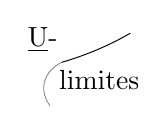
\begin{tikzpicture}[baseline=(p28limites.base),x=1cm,y=1cm]
\node[anchor=base west,inner sep=0pt] (p28limites) at (0,0) {limites};
\node[anchor=base west,inner sep=0pt] at (-.40,.55) {\inserted{$\underline{\mathrm{U}}$-}};
\draw[gray,line width=.3pt] (-.11,-.20) .. controls (-.27,.02) and (-.17,.25) .. (.04,.35);
\draw[line width=.35pt] (.04,.35) .. controls (.38,.45) and (.67,.58) .. (.91,.72);
\end{tikzpicture}
projectives (resp. aux $\underline{\mathrm{U}}$-limites inductives). \deleted{\begin{tikzpicture}[baseline=(p28dailleurs.base),x=1cm,y=1cm]
\node[anchor=base west,inner sep=0pt] (p28dailleurs) at (0,0) {\unsure{D'ailleurs}};
\node[anchor=base west,inner sep=0pt] at (1.45,-.10) {\unsure{\begin{tikzpicture}[x=1cm,y=1cm]\draw[gray,line width=.3pt] (0,0) .. controls (.12,-.06) and (.20,-.18) .. (.35,-.18);\end{tikzpicture}}};
\end{tikzpicture}, c'est une conséquence immédiate de 1.2.\unsure{(iii)|(ii)|(i)|(iii|(ii|(i}}}
% The last subdivision is heavily cancelled at the right edge; both stroke count and closing-parenthesis visibility remain doubtful.
% The right edge after droite is cropped; no unseen closing parenthesis has been added there.
% The faint extra lower-right tail at cancelled D'ailleurs is separate from the long cancellation stroke.
\figure{\begin{tikzpicture}[remember picture,overlay]
\coordinate (p28cancelmid) at (5.0,.85);
\coordinate (p28cancelend) at (4.72,-.25);
\draw[line width=.4pt] (p28cancelstart) .. controls +(-.45,-3.1) and +(.65,6.0) .. (p28cancelmid);
\draw[gray,line width=.3pt] (p28cancelmid) .. controls +(0,-.25) and +(.12,.25) .. (p28cancelend);
\node[anchor=west,inner sep=0pt] at (p28cancelend) {\unsure{}};
% Pale lower continuation: cancellation ink versus coincident surface trace remains open.
\end{tikzpicture}}
